%xelatex
\documentclass{article}
\usepackage[margin=0.6in]{geometry}
\usepackage{xltxtra}
\usepackage{xgreek}
\usepackage{listing}
\setmainfont[Mapping=tex-text]{Kerkis}
\usepackage[colorlinks=true,linkcolor=black,urlcolor=blue]{hyperref}
\title{Παράλληλη επεξεργασία}
\author{Μπαντολας Πέτρος 5028\\Σειμένης Σπύρος 5070\\Καλλιβωκάς Δημήτριος 4993}

\begin{document}
\maketitle
\section{Ανάλυση σειριακής έκδοσης}
Η συμπεριφορά της σειριακής εκδοσης έγινε με την χρήση του εργαλείου scalasca.
\begin{center}
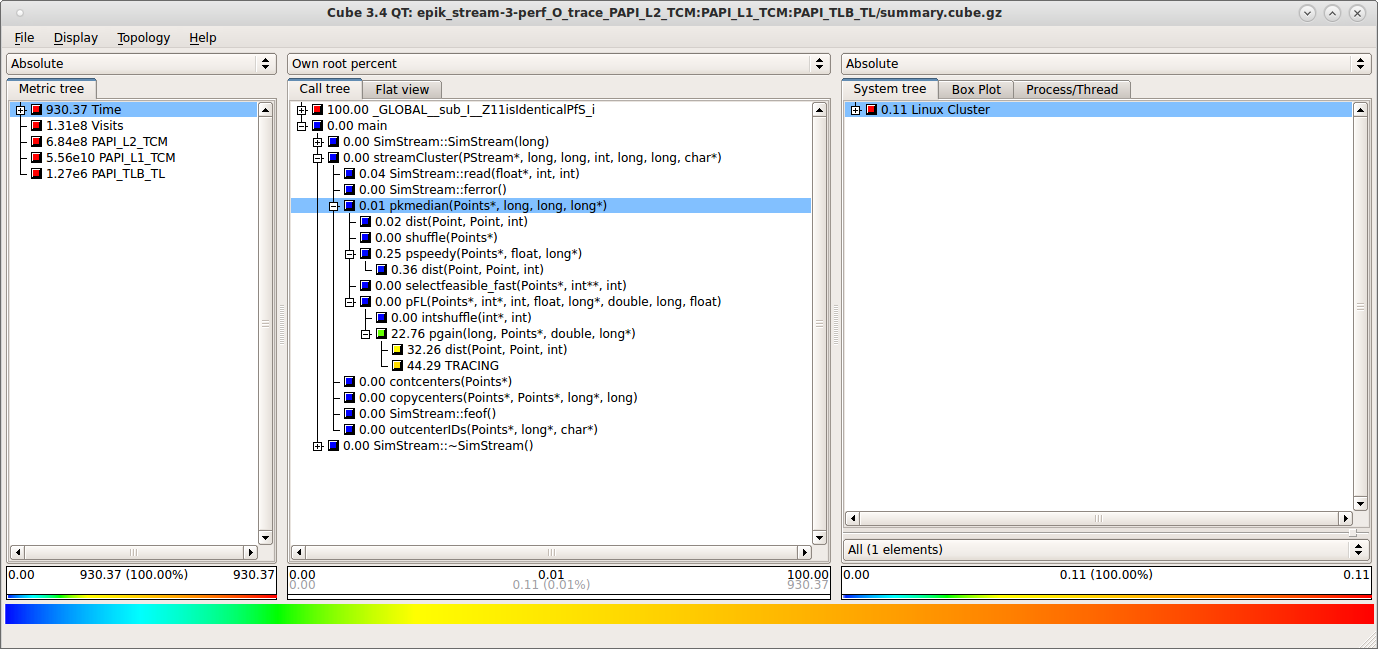
\includegraphics[scale=0.5]{../scrshots/time.png}
\end{center} 
Όπως φαινεται και στην εικόνα, οι συναρτήσεις με τον μεγαλύτερο χρόνο εκτέλεσης ειναι η pspeedy και η pgain.\\
Συγκεκριμένα ο μεγαλύτερος χρόνος και των δύο είναι κατα τις κλήσεις τους στην συνάρτηση dist.
\subsection{pgain}
Παρακάτω φαίνονται τα L1, L2, TLB cache misses της σειριακής έκδοσης όπου επι το πλείστον οφείλονται στην pgain.
\begin{center}
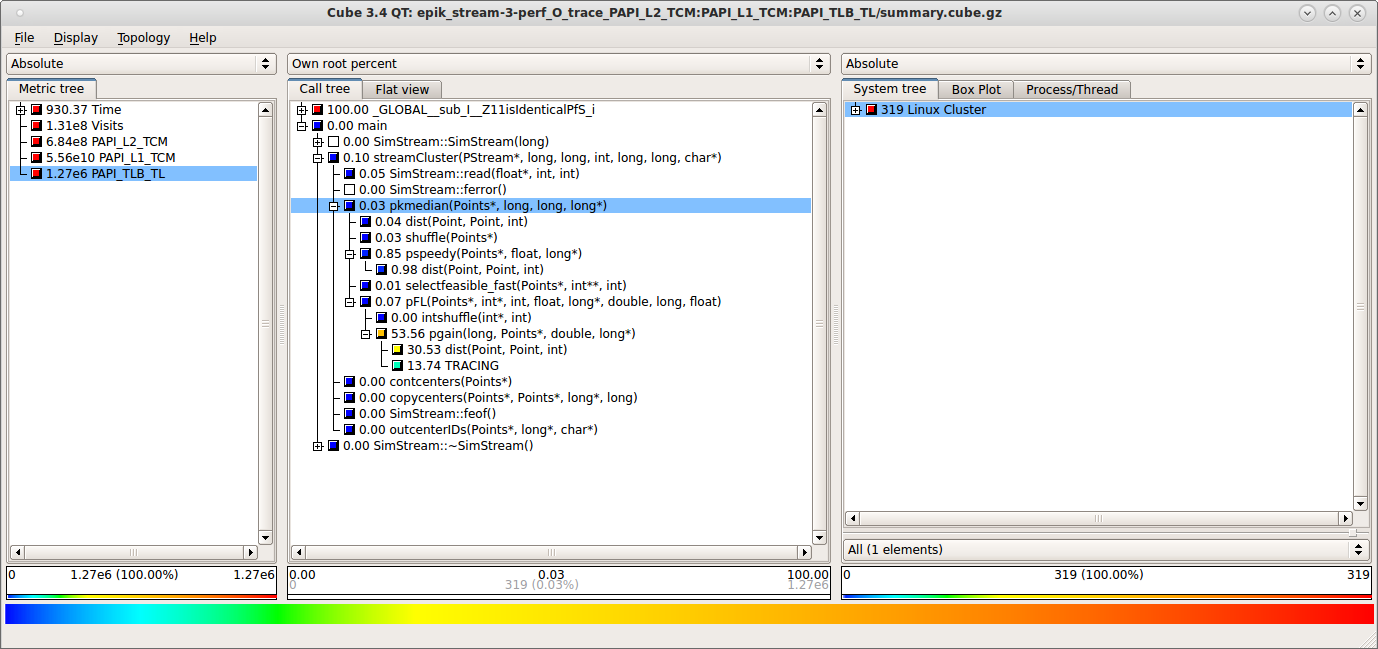
\includegraphics[scale=0.4]{../scrshots/tlb.png}
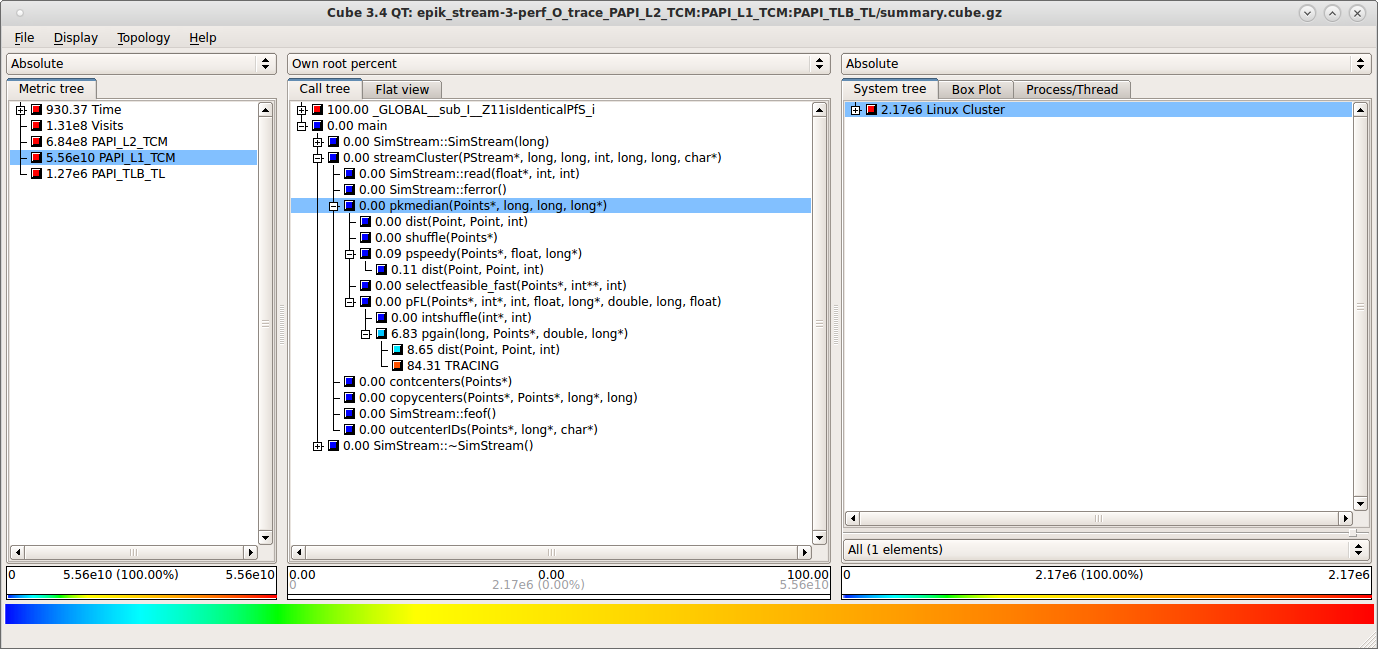
\includegraphics[scale=0.4]{../scrshots/l1.png}
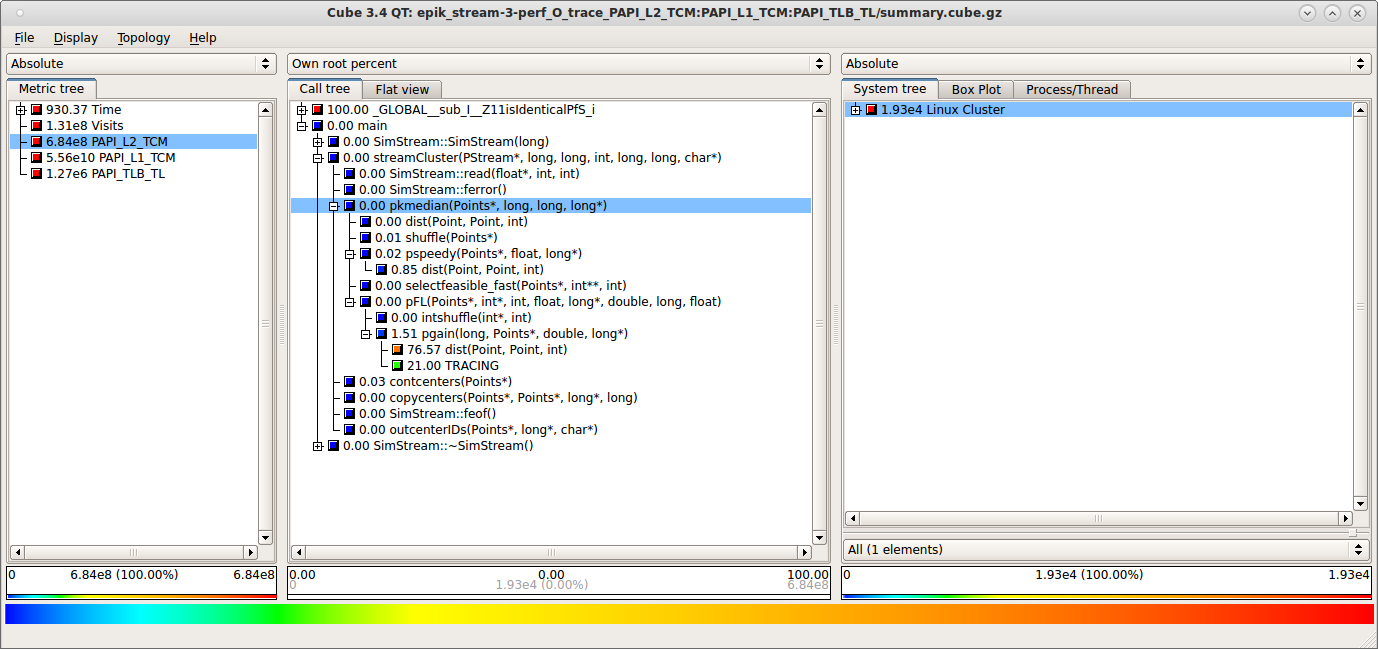
\includegraphics[scale=0.4]{../scrshots/l2.png}
\end{center} 
Συμπεραίνουμε οτι οι περιοχές που προκαλούν καθυστέρηση είναι αυτές που υπολογίζουν κατ' επανάληψη για όλα τα σημεία την απόσταση τους(dist). Η δομή που αποθηκεύει τα σημεία δεσμεύεται στην αρχή του προγράμματος στο heap μεσω malloc που δεν εγγυάται ότι οι διευθύνσεις φυσικής μνήμης θα είναι γειτονικες μεταξυ τους. Η πολλαπλή προσπέλαση όλων των σημείων σειριακά οδηγεί στα πολλαπλά cache misses. Έτσι η παραλληλοποίηση με openmp βελτιστοποιεί τους υπολογισμούς μειώνοντας τα cache misses.

\section{Παραλληλοποίηση}
\subsection{Με χρήση OpenMP}
-ΑΙΤΙΟΛΟΓΗΣΗ ΠΑΡΑΛΛΗΛΟΠΟΙΗΣΗΣ
-ΜΕΤΡΗΣΕΙΣ

\subsection{Με χρήση εντολών SIMD}
-ΑΙΤΙΟΛΟΓΗΣΗ ΒΕΛΤΙΣΤΟΠΟΙΗΣΗΣ
-ΜΕΤΡΗΣΕΙΣ






\end{document}



